
\chapter[Implementation]{Implementation}
\graphicspath{ {images/implementation} }
In this chapter, we present how we designed and implemented SYN, a tool that supports the software evolution comprehension approach 
defined in \autoref{s:EvolutionModel} and \autoref{s:3DRepr}. 

% In section x, we provide an overview of our platform by looking at all the modules that compose the architecture. 
% In section x, we present the tool's user interface, and finally, in section x, we detail how we implemented the auditory part. 

\section{Platform overview}

SYN is a platform tool that allows developers to have a visual and auditive depiction of an evolving system. 
It was designed to be extensible and efficient. The platform is composed of a set of modules, each one with its responsibility:
\begin{itemize}
    \item \textbf{SYN Core}: the core module, required by other modules. It holds classes representing basic SYN concepts such as ProjectHistories, ProjectVersions, and FileVersions. It also provides abstract classes, open to any implementation, to achieve the extensibility goal.
    \item \textbf{SYN CLI}: responsible for providing a Command Line Interface (CLI) interaction to users.
    \item \textbf{SYN Analyzer}: implements the analysis approach described in section \ref{s:EvolutionModel}. 
    \item \textbf{SYN Server}: provides GraphQL endpoints to retrieve data from SYN and display them in a user interface. 
    \item \textbf{SYN Debugger}: the user interface of SYN developed to debug and visually depict information collected during the analysis. 
\end{itemize}

All the modules of SYN are written in Java, except SYN Debugger, which is written with React and TypeScript. 

The modular architecture of SYN allows the user to interact with the tool in two ways: through the console with the commands provided by the SYN CLI module 
or through a web application embedded inside the SYN Debugger module. \\
\autoref{fig:architecture} gives a high-level overview of the architecture. Each row represents the dependencies between modules.
The heart of the system is the SYN Core module. It specifies concepts described in our approach and provides classes to standardize the communication between modules.
There is also a class called ViewGenerator, embedded in the core, which other modules use to create views over the collected repository's data.
The SYN Analyzer module carries out the analysis task; internally, it has classes that act as a repository explorer to retrieve data from the repository history. 
Moreover, metrics are extracted with the metrics extractor component and put inside the internal historical representation through the history builder component. 
Since we wanted to provide direct access to the analysis capabilities of SYN, the SYN CLI provides commands that directly call functions defined inside SYN Analyzer. 
This is why it has both SYN Core and SYN Analyzer as dependencies. 

SYN Debugger holds the GUI of SYN to represent a view graphically. Information is retrieved through endpoints specified by the GraphQL server of the SYN Server module, which, in turn, retrieves view data from the SYN Core module. 


\begin{figure}
    \center
    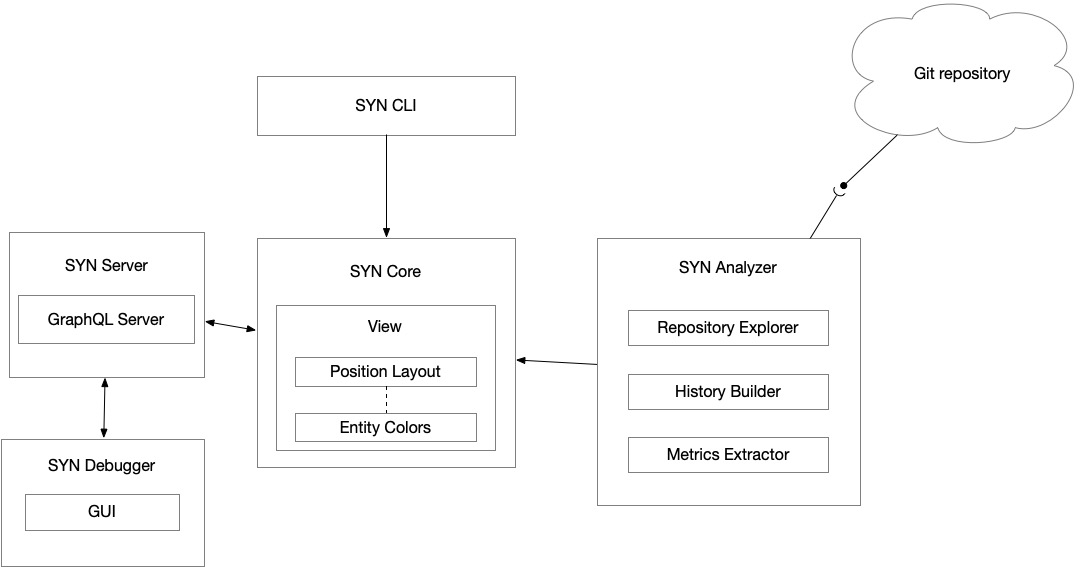
\includegraphics[width=\textwidth]{SYNArchitecture.jpg}
    \caption{Architecture of SYN}
    \label{fig:architecture}
\end{figure}

Having reached a low coupling between modules, the extensibility of SYN is preserved. Modules such as SYN Server or SYN Analyzer implementation could be changed without altering the codebase of other modules. 

\section{SYN Core}
SYN Core is the module that holds all the entities that we have introduced in \autoref{s:EvolutionModel}. 
All the classes of our abstraction extend the \texttt{Entity} class, composed of the field \texttt{id}, unique and used to identify an object inside our domain. 
To quickly identify the object type, each class has an identifier that makes the id prefix. 
Classes inside the model of SYN Core could be partitioned into four subdomains: Project, History, Analysis, and View. 

\subsection*{Project}
The first part of the model consists of the \textbf{Project} entities. 
The diagram is shown in \autoref{fig:SYNCLass}. The abstract class \texttt{Project} represents a software system. It defines the following fields:
\begin{itemize}
    \item \texttt{name}
    \item \texttt{projectHistory}: an object that represents the project's history. It holds the results of the analysis. 
    \item \texttt{path}: the path of the analyzed git repository. 
\end{itemize}

Moreover, we defined two additional classes \texttt{LocalProject} to represent a project present in the local storage and \texttt{RemoteProject} to describe a project that needs to be retrieved from a remote source. 
Therefore, if, on the one hand, \texttt{LocalProject} does not need any further fields to represent a local project, on the other hand, \texttt{RemoteProject} needs at least the \texttt{projectURL} field. We might add more information, such as the git branch or the remote credentials; despite that, we decided to keep the implementation as simple as possible. 


\begin{figure}
    \center
    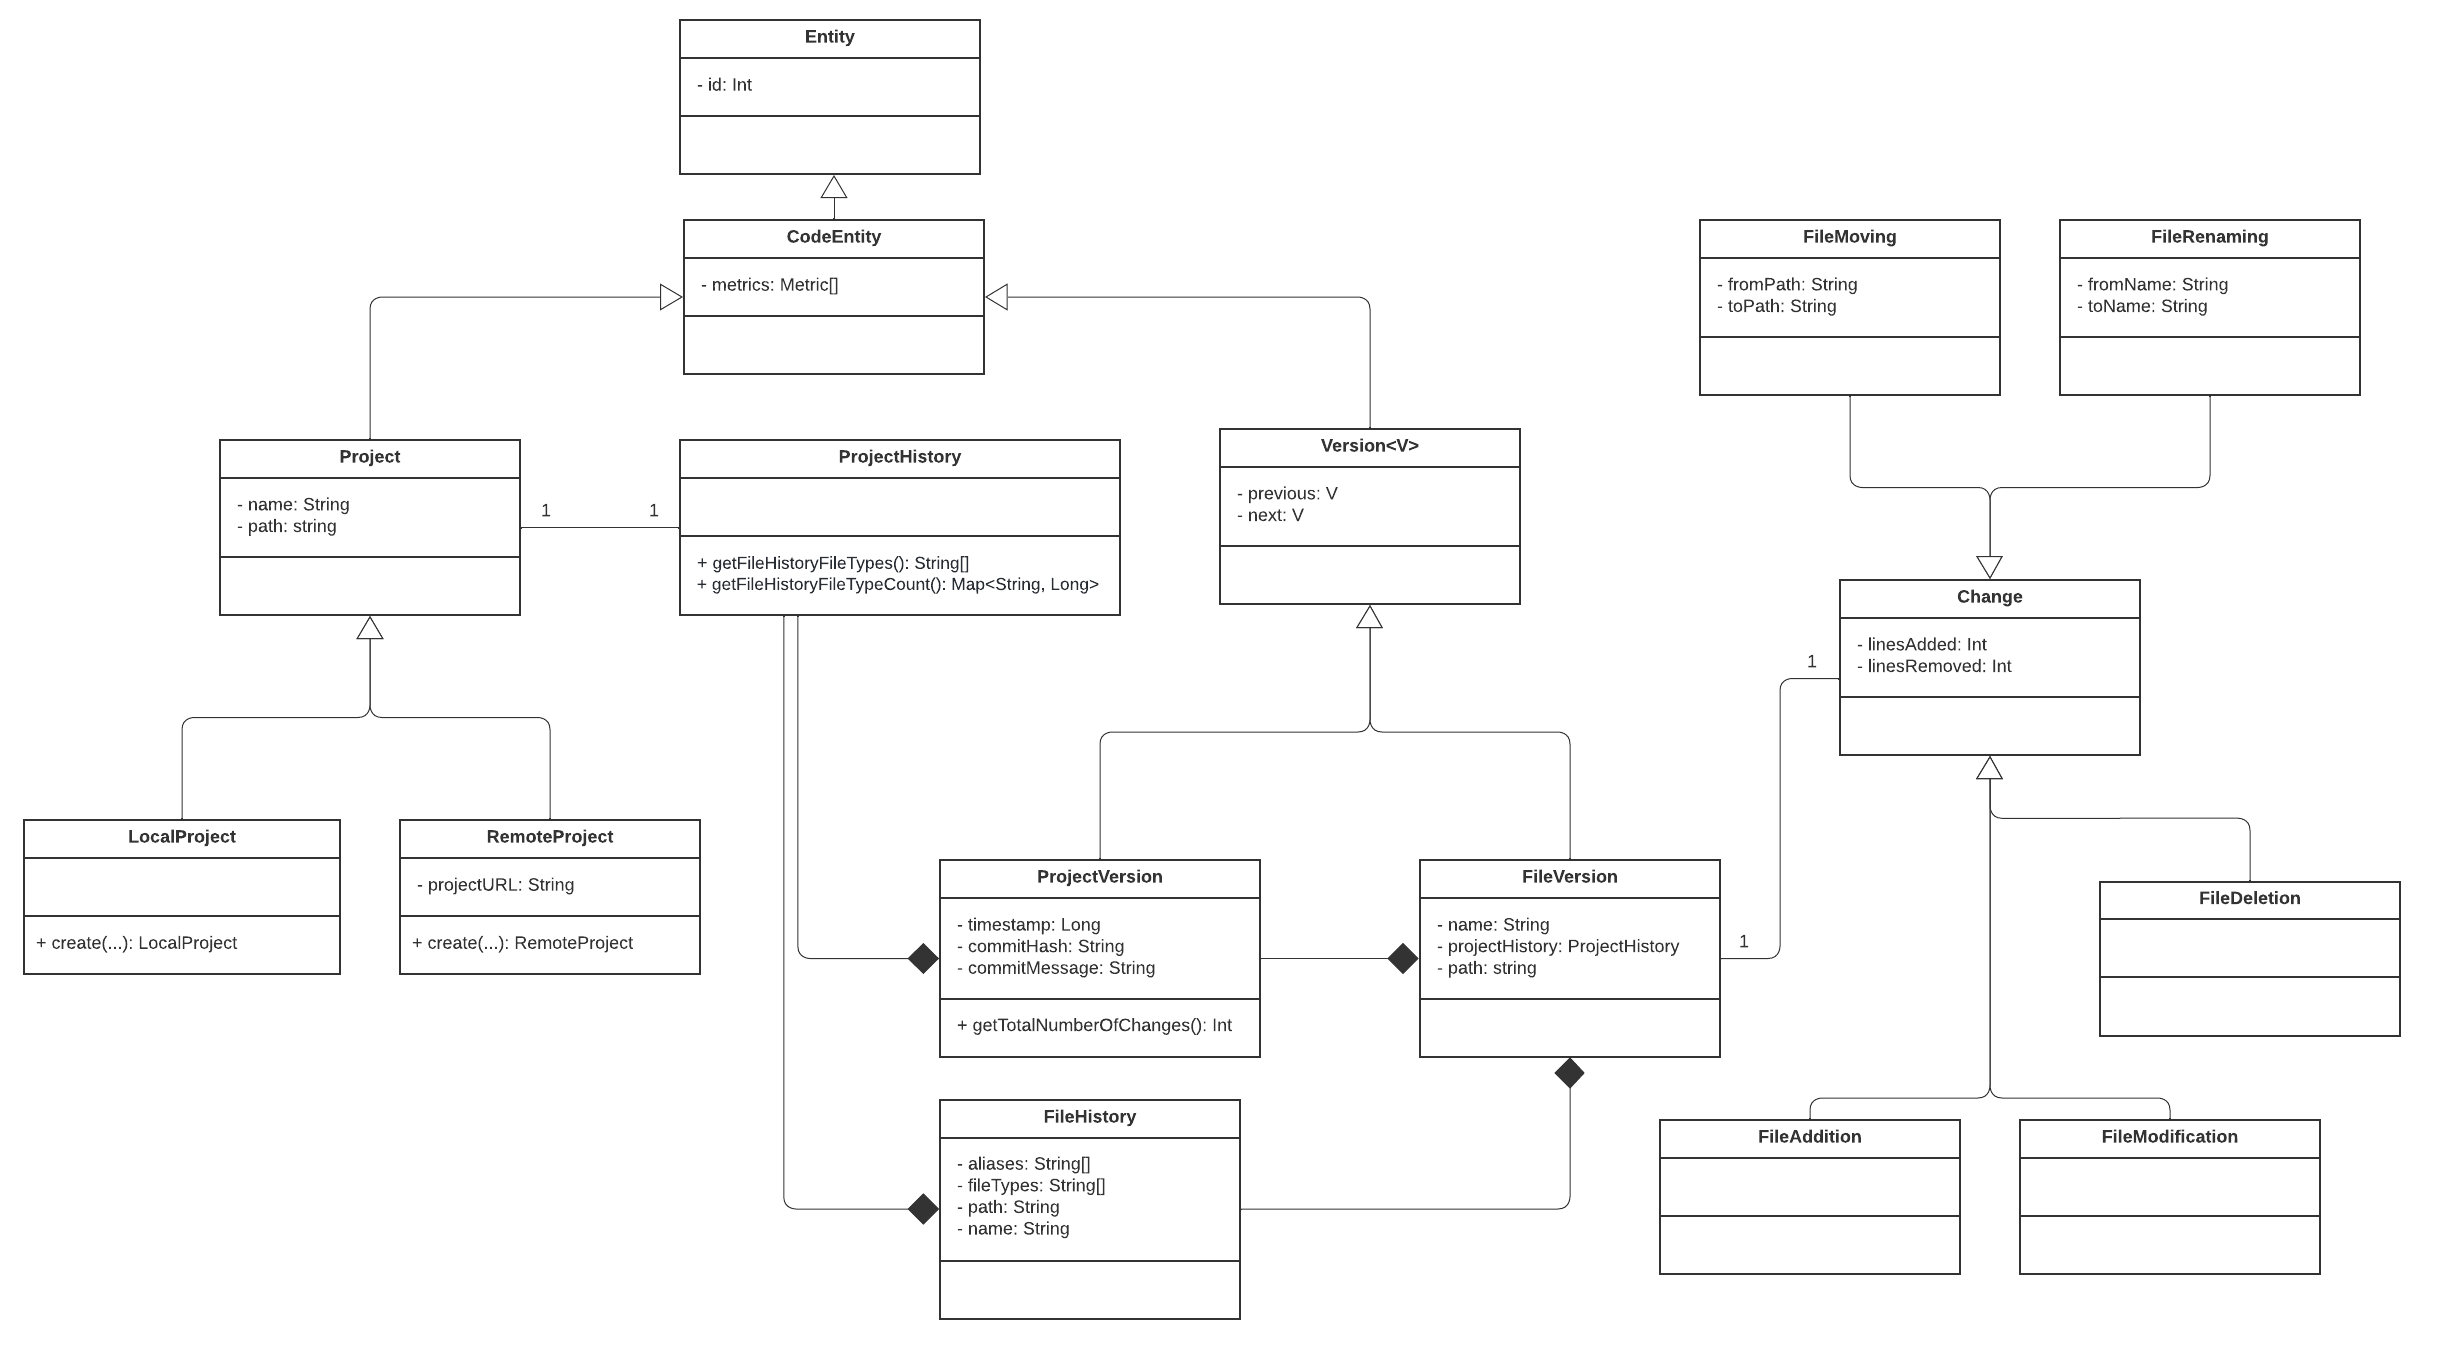
\includegraphics[width=\textwidth]{SYNClass.png}
    \caption{Class diagram of Project entities}
    \label{fig:SYNCLass}
\end{figure}

\subsection*{History}

As evidenced above, each project might hold a \textbf{ProjectHistory} object representing its history. 
Following what we have explained in \autoref{s:EvolutionModel}, the \texttt{ProjectHistory} class holds a group of ProjectVersion and a group of FileHistories. The \texttt{FileHistory} class, which represents the history of a single file, has the following fields:
\begin{itemize}
    \item \texttt{aliases}: a list of paths related to the file. We know that a single unique path identifies a file. However, since our approach is tolerant of moving and renaming activities, we have to store all the paths a file had. In \autoref{sec:SYNAnalyzer} we explain the importance of this field and why it has such a crucial role in our analysis. 
    \item \texttt{fileTypes}: A set of Strings representing each one representing a possible type of the file. 
    \item \texttt{path}
    \item \texttt{name}
    \item \texttt{fileVersions}: a list of FileVersions related to this FileHistory. 
\end{itemize}
With the \texttt{Version<V>} class, we want to represent the state of an entity at a particular point in time. 
The generic parameter \texttt{V} is used as a constraint to ensure the consistency of the class with the previous and the next versions. 
The \texttt{ProjectVersion} class is used to represent git commits; it defines the following fields: 
\begin{itemize}
    \item \texttt{fileVersions}: a list of FileVersions that are part of this commit.
    \item \texttt{timestamp}: expressed in seconds. 
    \item \texttt{commitHash}: hash of the commit generated by git when the commit was made and used to identify a commit uniquely. 
    \item \texttt{commitMessage}: the message written by the commit author when it was made. 
\end{itemize}
Extending the Version class, the ProjectVersion class also inherits the previous and next field that could be used to navigate through the history, similarly to how we traverse a LinkedList. 
Finally, the \texttt{FileVersion} class has the following fields:
\begin{itemize}
    \item \texttt{parentProjectVersion}: the ProjectVersion holding this FileVersion instance. It retrieves the commit's related information, such as the timestamp or the message. 
    \item \texttt{change}: represents the action made on that file. 
    \item \texttt{fileHistory}: represents the file being modified. 
\end{itemize}

In our approach, we have identified five different types of changes. They were implemented by extending the \texttt{Change} class, as depicted in \autoref{fig:SYNCLass}. The Change class declares two fields, \texttt{linesAdded} and \texttt{linesRemoved}, each one representing the number of lines added and, in turn, removed. 
The goal of our model is to be easily extensible. With that in mind, if in a future implementation, we want to extend the variety of metrics specifically collected for each kind of change, we need to extend the relative class, and the polymorphic mechanisms of Java will do the rest. 

An example of that can be seen in the class \texttt{FileMoving} or in the class \texttt{FileRenaming}, which specifies two fields to track the previous and the next path after the change. 




\subsection*{Analysis}
Even though the analysis is effectively implemented into another module, SYN Core provides some abstract classes that need to be implemented to allow the exchange of analysis results. 
The first class that the model defines is \textbf{AnalysisWorkDescriptor}.
As the name suggests, it is a holder of helpful information to instruct the analyzer on what it has to do. This information comprehends the project we have to run the analysis and the list of commits that must be analyzed. 
The reason for this implementation choice is to allow multiple threads to run in parallel analyses without analyzing the same commit numerous times. 
We described this approach in \autoref{s:partialHistoricalRepr}.
\bigbreak

Inside the core module we also have the \textbf{FileTypeManager} class. It is responsible for mapping a set of functions to compute evolutionary metrics. We implemented the metrics presented in \autoref{s:evolutionaryMetrics}. However, any external module could easily extend this set of functions. This choice allowed external components to increase the set of metrics computed in SYN. Therefore, the analysis can be customized to collect relevant metrics for a specific project. Once the function to extract a metric given a File is written, the developer must associate it with the corresponding FileType. For example, if in the future an engineer wants to write an  Object-Oriented (OO) metric, such as the number of parents, they can create a function to compute it and associate the function to the OO type.
\bigbreak

Finally, in our model, we also defined the \textbf{ProjectAnalysisResult} class. An analyzer must use it to return the results that it collected. In addition, this class made a distinction between partial and total analysis results, allowing it to be used with the partial history retrieval approach defined in \autoref{s:partialHistoricalRepr}. The fields declared in this class are:
\begin{itemize}
    \item \texttt{project}: the projects on which the analysis was done.
    \item \texttt{analysisCompleted}: whether the analysis is partial or total.
    \item \texttt{timestamp}: the timestamp when the analysis was done. 
    \item \texttt{firstCommit}: the first commit considered in this analysis. 
    \item \texttt{lastCommit}: the last commit considered in this analysis. 
    \item \texttt{projectVersions}: a list of ProjectVersion discovered during the analysis.
    \item \texttt{fileHistories}: a list of FileHistories discovered during the analysis.
    \item \texttt{fileVersions}: a list of FileVersions discovered during the analysis.
\end{itemize}

Moreover, this module also provides an abstraction of the core concepts of the Git protocol. It defines the \texttt{GitProject}, \texttt{GitCommit} and \texttt{GitChange} classes, each one respectively representing a repository, a commit, and a change on a file. 
Thanks to this choice, each external module can provide a way to retrieve data from a git repository without having to share internal classes or dependencies with other modules. 


\subsection*{View}
\label{s:view_impl}
In \autoref{s:3DRepr} we explained our visual approach. To implement it, we have defined a class called \textbf{View}, that designates how the visualization should be rendered. 
In our visualization approach, we have to display the evolution of a repository. To do that, the user interface must sequentially display a list of AnimationFrames, each representing a state of the repository at a particular time. We designed the class \textbf{ViewAnimation} to define a frame of the view animation. This class has two properties:
\begin{itemize}
    \item \texttt{representedEntities}: a list of ProjectVersions whose data had been used to create that frame.
    \item \texttt{viewFigureList}: a list of ViewFigure each one representing a FileHistory in the view.
\end{itemize}

The \textbf{ViewFigure} class holds graphical properties to properly display each FileHistory
\begin{itemize}
    \item \texttt{position}: the position of the entity.
    \item \texttt{color}: the color of the entity.
    \item \texttt{height}: the height of the entity.
    \item \texttt{shape}: a literal that represents the shape of the entity. 
    \item \texttt{age}: the age of the entity.
    \item \texttt{enabled}: wether the enity should be visualized or not.
    \item \texttt{opacity}: the opacity of the entity.
    \item \texttt{size}: the size of the entity.
\end{itemize}

These properties are computed when the \texttt{View} object is instantiated. A view is created on the top of the user's preferences. 
So, for example, if the user wants to use a specific color for a particular action, like the dark green for the additions, we have to store this information somewhere. 
This is why we defined the \textbf{ViewSpecification} class. A \texttt{View Specification} is the crucial element of each view. 
All the views are generated from a \texttt{ViewSpecification} instance. The list of available properties defined inside a \texttt{ViewSpecification} are:
\begin{itemize}
    \item \texttt{versionGroupingStrategy}: the strategy that SYN needs to follow to group up commits and create moments.
    \item \texttt{versionGroupingChunkSize}: the dimension of each group; it can be several commits or an amount of time. 
    \item \texttt{colorPalette}: the mapping that SYN has to follow to map FileVersion's actions to colors. 
    \item \texttt{agingGroupingStrategy}: the strategy that SYN needs to follow to define an age.
    \item \texttt{agingStepSize}: the dimension of each age; it can be a number of commits or an amount of time. 
    \item \texttt{agingSteps}: the number of available aging steps. 
    \item \texttt{mapperStrategy}: the strategy that SYN has to follow to compute the height of each entity.
    \item \texttt{mapperStrategyOptions}: optional properties of the mapper if needed.
    \item \texttt{mapperMetricName}: the metric that the mapper should consider to compute the height. 
    \item \texttt{showUnmappedEntities}: wether the view should display entities without the selected metric.
    \item \texttt{fileTypeShape}: the mapping that SYN has to follow to associate a FileType with a shape.
    \item \texttt{fileTypeOpacity}: the mapping that SYN has to follow to associate a FileType with an opacity level.
    \item \texttt{figureSize}: the size of each figure.
    \item \texttt{figureSpacing}: the space between each figure.
    \item \texttt{showDeletedEntities}: wether the view should display deleted eneitites.
    \item \texttt{withGround}: wether the view should include a ground element.
\end{itemize}

Moreover, we defined an abstract class \textbf{PositionLayout} whose implementation specifies how entities should be laid out and a class \textbf{MapperStrategy} whose implementation specifies how the height of the entity is computed. The set of the mapping function is extensible. To implement a strategy a developer needs to implement an interface that defines two methods: \texttt{void generateStrategy(final List<String> values)} and \texttt{double mapValue(final String value)}. The mapping process is composed of two phases:
\begin{itemize}
    \item Generation phase: when the view is created, the method \texttt{generateStrategy} is called with all the values of the chosen metric. 
    \item Retrieve phase: when a new ViewFigure is created, the value of its height is set as the return value of the function \texttt{mapValue} given as an argument the value of the chosen metric for that file on that AnimationFrame. 
\end{itemize}

In our initial implementation, we provided five different mapping strategies:
\begin{itemize}
    \item LinearMapperStrategy: this strategy adopt a linear function internally to retrieve the height of a ViewFigure. 
    \item NormalizerMapperStrategy: during the generation phases, all the values are normalized in an interval between zero and one.

    \item BucketCountStrategy: during the generation phases, all the values are partitioned into buckets. The value returned by this function is the number of the bucket where the value was put. This strategy allows the customization of the number of buckets that are created. By default, this value is set to 100. 
    \item BucketValueStrategy: relies on the BucketCountStrategy. During the generation, duplicate values are removed to equally distribute buckets over the range of values recorded by the chosen metric. 

    \item LinearBucketValueStrategy: relies on the BucketValueStrategy. During the generation phase, the maximum value of each bucket is recorded. Therefore, during the retrieved phase, it is used to make a liner proportion of the value and add them to the bucket number. For example, assuming that values $100, 200, 500$ are mapped to the bucket $3$; therefore the value of $100$ is computed as $3 + 100/500 = 3.2$, the value of $200$ is $3 + 200/500 = 3.4$ and finally the value of $500$ is $3 + 500/500 = 4$.
\end{itemize}



\section{SYN CLI}
SYN CLI is a command-line interface that allows developers to interact with SYN. It gives developers complete control over the system.
\bigbreak
\textbf{Analysis commands}
\bigbreak

\lstinline{syn analyze auto -p <project_id> -o <output_file> -t <thread_count>}\\
\\
This command is used to run an automatic analysis with SYN. 
Given the project's id, the system automatically creates \texttt{thread\_count} thread workers (5 by default), runs the analysis in parallel, and joins the results in the output file. 
Furthermore, this command ensures that each thread has a different git repository to work on. 
\bigbreak

\lstinline{syn analyze join -o <output_file> <...analysis_file>}\\
\\
This command is used to join analysis results into a single output file.
\bigbreak
\begin{lstlisting}
syn analyze manual -p <project_id> -g <git_repo_path>
    -rc <first_commit> -lc <last_commit> -o <output_file>
\end{lstlisting}
\bigbreak
This command is used to perform a manual analysis with SYN. This command lets the developer have the freedom to choose the repository path and both the first and the last commit of the analysis. 
If the first commit is not specified, the analysis starts from the beginning of the history, and, in the same way, if the last commit is not specified, the study ends with the end of the history. 
\bigbreak

\begin{lstlisting}
syn analyze prepare -p <project_id>  -g <git_repo_path> 
    -wn <workers_number> -of <output_folder>
\end{lstlisting}
\bigbreak
This command is used to create a folder of workers to analyze a project.
Based on the number of workers, the repository history is equally partitioned into chunks, each assigned to a worker. 
\bigbreak

\lstinline{syn analyze worker -p <project_id> -g <git_repo_path> -w <worker_file -o <output_file>}\\
\\
This command runs the analysis on a project given its worker file. 
Furthermore, here the user can specify the git path because two analyzers cannot use it simultaneously, so it is up to the user to choose a free git repository. 

\bigbreak
\textbf{Prioject commands}
\bigbreak

\lstinline{syn project list}\\
\\
This command is used to print a list of available projects in the console.

\bigbreak
\lstinline{syn project create -n <project_name> -p <project_location>}\\
\\
This command is used to create a project given its name and its location. The location could be either a path or an URL. 

\bigbreak
\lstinline{syn project inspect -g <git_path> <project_id> <FileHistory_id>}\\
\\
This command is used to inspect all the FileVersions of the indicated FileHistory. Furthermore, if the git repository is provided, SYN performs a double check to ensure that all the FileVersions were spotted. \
To do so, it exploits the output of the command "\lstinline{git log --full-history -- <FileHistory_path>}," keeping attention if the FileHistory's path was changed (git cannot do that).

\bigbreak
\lstinline{syn util csv <project_id> -o <output_file>}\\
\\
This command produces a CSV containing all the commit's tracked information of the selected project. 


\section{SYN Analyzer}
\label{sec:SYNAnalyzer}
The SYN Analyzer module implements the analysis approach described in section \ref{s:EvolutionModel}.
To walk through the git-tree, it uses a Java git adapter called JGit \footnote{\url{https://www.eclipse.org/jgit/}}. 
To do so, we extended Git classes provided by the SYN Core module, and we created the \texttt{JGitProject}, \texttt{JGitCommit} and \texttt{JGitChange} classes. Their job is to call the JGit API and retrieve historical information. 
\bigbreak

To run the analysis, we need to obtain first an \texttt{AnalysisWorkDescriptor}. 
In this module, we developed a class \texttt{JGitAnalysisWorkerDescriptorFactory} to partition the commit tree and obtain a set of workers. 
\autoref{fig:historysplit} shows an example of a partition with three workers. First, the whole history of git is retrieved and stored in memory. Secondly, all the branches' commits are merged into a single list sorted by their timestamp. 
Then, the merge commits are removed since the changes recored by them are duplicated and finally the resulting list is partitioned to match the requested number of workers. 
\begin{figure}
    \center
    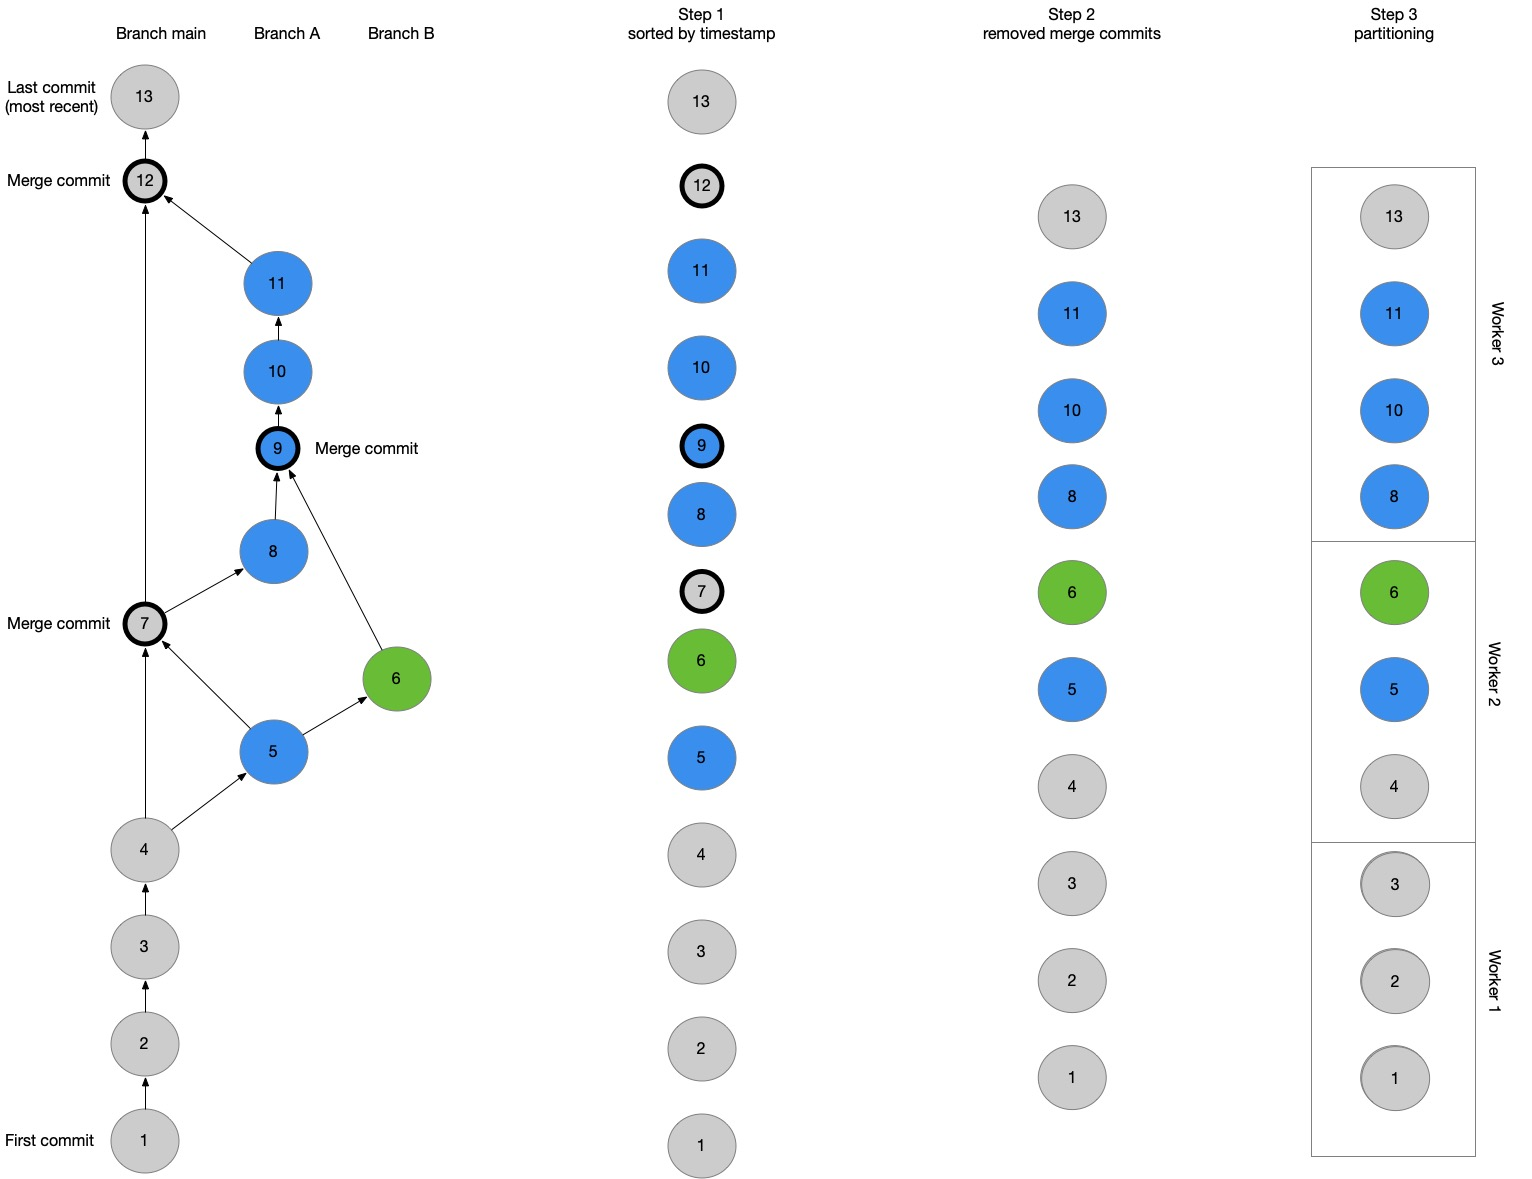
\includegraphics[width=\textwidth]{HistorySplit.jpg}
    \caption{Partition of the commit tree with 3 workers.}
    \label{fig:historysplit}
\end{figure}


The analysis process of a single worker contemplates the following steps:
\begin{enumerate}
    \item we call the method \texttt{runAnalysis} of the class \texttt{ProjectAnalyzer} with a worker descriptor and a project as an argument. 
    \item the analyzer reads the git path of the project and instantiates a new \texttt{GitProject}. 
    \item a list of commits, specified in the worker, is retrieved from the \texttt{GitProject}.
    \item the first commit of the list is retrieved, a new \texttt{ProjectVersion} is created with its details. 
    \item the analyzer runs the checkout command of git to restore the version of the system at the one specified by the commit. 
    \item the analyzer retrieves a list of modified files. 
    \item for each modified file, the analyzer creates a new \texttt{FileVersion}, links it with the corresponding  \texttt{ProjectVersion} and \texttt{FileHistory} (creates it if it does not exist yet), and finally extracts all the evolutionary metrics expected for that file type.
    \item once all the modified files are analyzed, the analyzer repeats steps 5, 6, and 7, considering the subsequent commit of the list each time. 
    \item once all the commits are analyzed, the analyzer returns all the discovered results within an \texttt{ProjectAnalysisResult} object. 
\end{enumerate}

\bigbreak
We have to run the analysis in parallel if we want to analyze a large repository in an acceptable amount of time. Therefore, with large git repositories, we might need many workers. We have said that each worker produces a \texttt{ProjectAnalysisResult} that represents a partial history. To obtain the entire history of the repository, we have to join all these partial analysis results. 
In SYN, each entity is identified by an id. 
The order in which entities are created is essential because we visually sort entities based on their creation timestamp. 
Therefore, having consistency between ids of FileHistory is the most crucial feature that a join algorithm must provide.
We said that each analysis result has: a list of \texttt{FileVersions}, a list of \texttt{ProjectVersions} and a list of \texttt{FileHistories}. 
Analyzers are not meant to communicate with each other. Therefore they work in isolation, like in a sandbox. 
When we have to join the results, the concatenation of the \texttt{FileVersions} or the \texttt{ProjectVersions} is not a problem if the historical sequence is respected. 
These objects are mutually independent of each other.
The challenge comes with the \texttt{FileHistories}. When the analyzer spots a file, if it was not discovered yet, it creates a new \texttt{FileHistory} with a unique id. 
This sounds like a problem with merging because we might consider the same file twice. In other words, we have an issue linking FileHistories between analysis results.
Assuming for a moment that we do not have this obstacle, another situation might happen, more tricky than the previous one. 
If in the middle of two analysis results, a file changed its path, on the first analysis, we have an entity with the old path, 
and on the second analysis, we have an entity with a new path. 
Unless we won't keep track of all the possible paths of an entity, it is impossible to reconstruct a connection between these two files. 
This is the reason that brought us to put the \texttt{aliases} field in the \texttt{FileHistory} class. 

In the join algorithm we developed, we employ a map to keep track of FileHistories.
As a result, nevertheless, the file has a different id on any analysis result, the consistency between
FileHistories is guaranteed. Furthermore, we can guarantee the absence of duplicates inside the newly built repository history. 

We present an algorithm that takes as input a list of already discovered FileHistories and an \texttt{ProjectAnalysisResult} and it returns a dictionary.
This dictionary is used to map partialFileHistories, the FileHistory of an analysis result, to definitiveFileHistories, which are part of the entire history of the repository. 
To obtain this map, it uses the following strategy:
\begin{enumerate}
    \item If the last alias of a definitiveFileHistories is equal to the first alias of a partialFileHistory, then they represent the same file.
    \item If in the partialAnalysisResult there is more than one FileHistory with the same first alias, only the first is mapped to a definitiveFileHistories, and the other partialAnalysisResult are mapped to a new FileHistory.
    \item If a partialFileHistory has not matched an alias with a previously created definitiveFileHistories, then it represents a new definitiveFileHistories.
\end{enumerate}

% \begin{algorithm}
%     \caption{Algorithm to create a mapping between partialFileHistories and definitiveFileHistories}
%     \label{alg:cap}
%     \begin{algorithmic}[1]
        
%     \State $partialToDefinitiveMap \gets new Map()$
%     \State $partialAliasToFileHistory \gets new Map()$
%     \State $newFileHistories \gets new List()$
%     \end{algorithmic}
% \end{algorithm}

\begin{algorithm}
    \caption{Algorithm to create a mapping between partialFileHistories and definitiveFileHistories}
    \begin{algorithmic}[1]
    \Procedure{PartialToDefinitiveFH}{$projectAnalysisResult, partialFileHistories$}
        \State $partialToDefinitive \gets Map()$
        \State $partialAliasToFH \gets Map()$ \Comment{Strategy 1}
        \State $unmappedPartialFileHistories \gets List()$  \Comment{Strategy 2}
        \ForAll{partialFH in partialFileHistories}
            \State $firstAlias \gets partialFH.aliases[0]$
            \If{$!partialAliasToFH.has(firstAlias)$}
                \State $partialAliasToFH.set(firstAlias, partialFH)$  \Comment{Strategy 1}
            \Else
                \State $unmappedPartialFH.append(partialAliasToFH)$  \Comment{Strategy 2}
            \EndIf
        \EndFor

        \ForAll{definitiveFH in projectAnalysisResult} \Comment{Strategy 1}
            \State $lastAlias \gets definitiveFH.aliases[definitiveFH.length - 1]$
            \If{$partialAliasToFH.has(lastAlias)$}
                \State $partialFH = partialAliasToFH.get(lastAlias)$
                \State $definitiveFH.path = partialFH.path$
                \State $definitiveFH.aliases.addAll(partialFH.aliases)$
                \State $partialToDefinitive.set(partialFH, definitiveFH)$
                \State $partialAliasToFH.remove(lastAlias)$
            \EndIf
        \EndFor

        \State $unmappedPartialFH.addAll(partialAliasToFH)$ \Comment{Strategy 3}
        \ForAll{partialFH in unmappedPartialFH} 
            \State $definitiveFH = FileHistory(partial.name, partial.path)$
            \State $definitiveFH.aliases = partialFH.aliases $
            \State $partialToDefinitive.set(partialFH, definitiveFH)$
        \EndFor
        \State \textbf{return} $partialToDefinitive$
    \EndProcedure
    \end{algorithmic}
\end{algorithm}


\section{SYN Server}
SYN Server is responsible for providing the elaborated information, given by the analysis results, in an intermediate language between the 
front-end (SYN Debugger) and the back-end. We used SpringBoot, a Spring-based tool for efficiently developing "production-ready" applications.

\subsection*{GraphQL API} 
The server module provides a set of GraphQL endpoints to retrieve information from SYN. 
GraphQL is a query language for APIs that allows clients to ask for exactly what they need.
This is an advantage compared to a REST API because, instead of always returning a predefined set of data, GraphQL only returns the needed information, making the communication more effective. 
In GraphQL, endpoints are divided into queries and mutations. Queries are used to retrieve data, while modifications are used to create or alter data. 

\bigbreak
\textbf{Mutations}

=> \texttt{createProject(projectName: String!, projectLocation: String!): Project} 
used to create and automatically analyze a new project.
It takes as parameters the name of the project and its location (the path on the local machine or the URL) as a String. 

\bigbreak
\textbf{Queries}

\texttt{projectList:  [PartialProjectInformation]!} \\ 
is used to retrieve a list of projects. For performance reasons, with this query only the name and the id of a project can be retrieved. 
\bigbreak
\texttt{view(projectId: Int!, viewSpecification: ViewSpecificationInput!): View} \\
returns a view of the project identified by the argument \texttt{projectId}, built following the directives specified in the \texttt{viewSpecification} object. 
This query returns an object representing a view; thus, it has all the fields described in \autoref{s:view_impl}. 
\bigbreak
\texttt{partialView(projectId: Int!, viewSpecification: ViewSpecificationInput!, viewAnimationId: Int): View} \\
returns a view with only the next 100 AnimationFrames starting from the one identified by \texttt{viewAnimationId}. 
This endpoint was created to enable performance optimizations on clients. If the viewSpecification expected too many animations, the resulting view would be a bottleneck for the client.
With this endpoint it can still retrieve the view, and then animation can be lazily loaded once they are effectively required. 
\bigbreak
\texttt{fileHistory(projectId: Int!, fileHistoryId: Int!): FileHistory} \\
used to retrieve details of the FileHistory identified with \texttt{fileHistoryId} of the project identified with \texttt{projectId}.
\bigbreak
\texttt{projectVersions(projectId: Int!, projectVersionsId: [Int]!): [ProjectVersion]!} \\
used to retrieve details of the ProjectVersion identified with \texttt{projectVersionsId} of the project identified with \texttt{projectId}.
\bigbreak
\texttt{groupingPreview(projectId: Int!, viewSpecification: ViewSpecificationInput!): Int} \\
this endpoint is used to compute the number of AnimationFrames that are gonna be created with the given \texttt{viewSpecification}.
\bigbreak
\texttt{fileTypeCounter(projectId: Int!): [FileTypeCounter!]!} \\
this endpoint returns a list that maps each FileType with the number of occurrences that it has in the project \texttt{projectId}.
\bigbreak
\texttt{fileTypeMetrics(projectId: Int!, fileTypeFilter: [String]): [FileTypeMetrics!]!} \\
this endpoint returns a list that maps each FileType with a list of metrics available for it. Only the FileTypes specified in the \texttt{fileTypeFilter} list are considered. 



\begin{figure}
    \center
    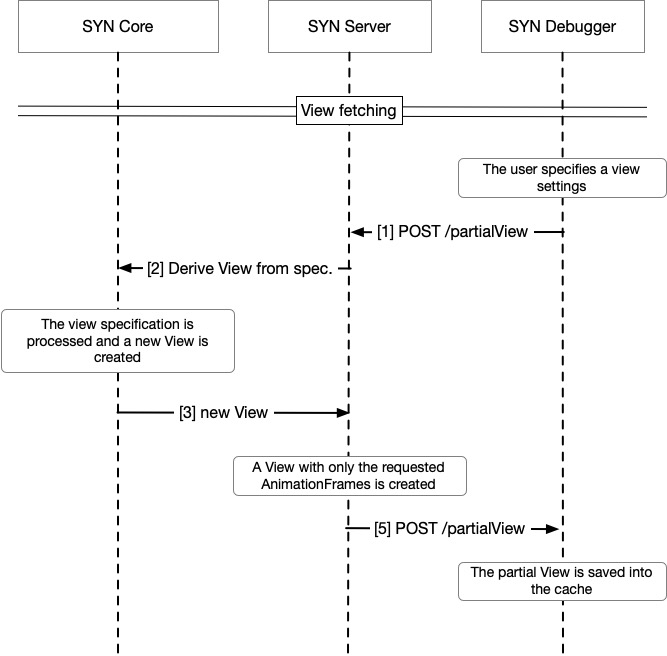
\includegraphics[width=\textwidth]{ServertClientFlow.jpg}
    \caption{Example of how a view is retrieved through GraphQL}
    \label{fig:ServertClientFlow}
\end{figure}

\bigbreak
\autoref{fig:ServertClientFlow} explains how a View is retrieved through a GraphQL endpoint with a sequence diagram. Once the client, in this case, SYN Debugger, has specified a \texttt{viewSpecification}, it makes a POST request to the 
\texttt{partialView} endpoint specifying the \texttt{projectId} requested, the \texttt{viewSpecification} and the \texttt{viewAnimationId} of the AnimationFrame needed. SYN server, in turn, makes the same request to the SYN Core module. A new View is created and retrieved from SYN Server; it is modified to include only the AnimationFrames requested from the client. When the partialView is computed, it is returned to the client. 


\section{SYN Debugger}

SYN Debugger is a web application that allows developers to interact with SYN. It is written with React.js, a popular JavaScript framework. 
This application aims to have a visual depiction of the view generated by the server, plus some additional information. 
For example, it allows you to click on a file and see the related information. 
The visualization is based on Babylon.js, an open-source 3D library. 
SYN Debugger provides different kinds of customizations for the visualization, such as the entities' shape and colors. 
These customizations are sent to the back-end server through a {\em view specification} file as shown in \autoref{fig:ServertClientFlow}. 

The primary purpose of this application is to debug the view and explore all the possible visualization combinations of a system.
The main page of the visualization holds a list of projects.

\subsection*{Project setup}
When a project is selected, the UI searches a view specification in the web browser's local storage. 
The first view loaded is the project setup if it is not present.
The project setup is a view that allows the user to express preferences about how the UI should be rendered. 
Five steps compose this view:
\begin{itemize}
    \item Component selection: where the user can express which kind of FileType must be considered in the viewSpecification. 
    For each FileType, a counter representing how many FileHistories have that type is shown to ease the choice. 
    \item Grouping version strategy: enables the user to choose how moments should be created.
    \item Figure settings: to customize the shape, metrics, and opacity of each FileType. Moreover, with this view, the user can choose the mapping strategy for the height of entities. 
    \item View color: to customize the color of each change and how aging must act. 
    \item View settings: to customize some general settings such as the speed of the visualization, shadows or deleted entities should be kept. 
\end{itemize}

\subsubsection*{Component selection}
The first step of the setup, shown in \autoref{fig:SYNUIsettings1}, shows a list of cards, each representing a FileType. 
We can break the visualization area down into two parts: on the top one, there are two cards to represent binary files and text files. 
The sum of these two counters represents the total number of FileHistories present in the system because each file must be textual or binary. 
On the bottom are all the cards whose type is extracted by the extension of the file history. For example, if a file is named "foo.java" the JAVA card in this area represents it. 
Cards are sorted in descending order by their counter. This view considers all the FileType present in the system. To show the complete list, users have to click on the "show more."

\begin{figure}
    \center
    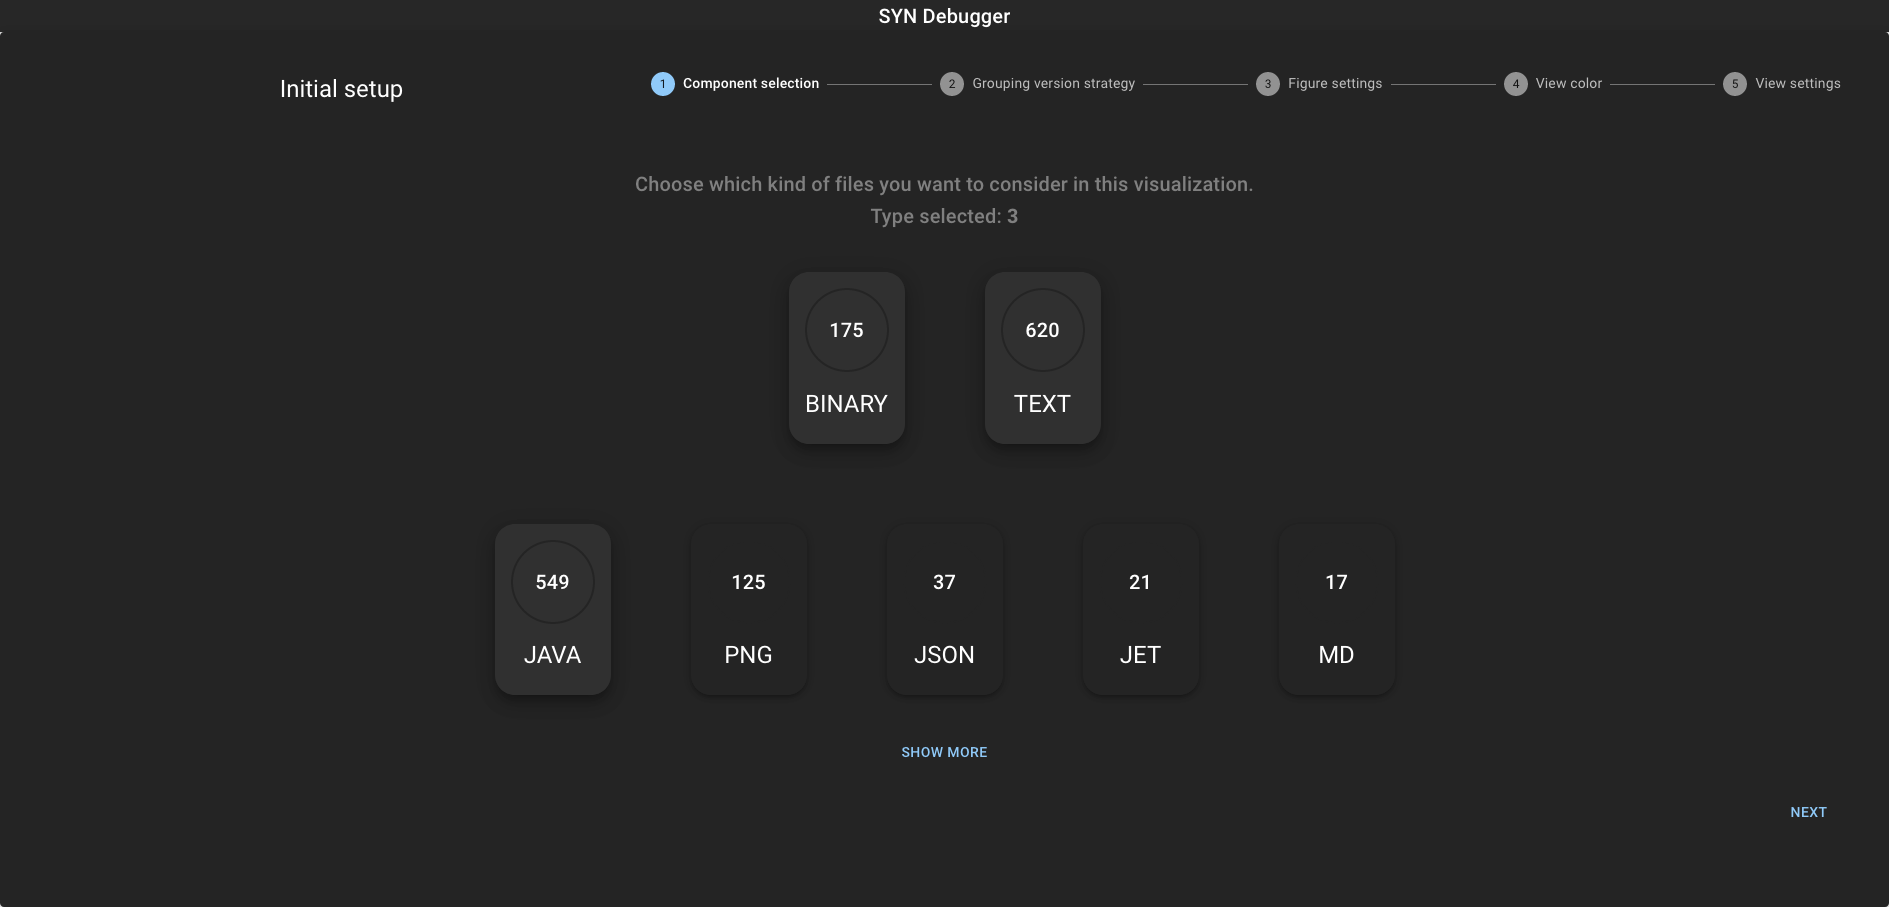
\includegraphics[width=\textwidth]{SYNUI-settings1.png}
    \caption{Project setup: component selection}
    \label{fig:SYNUIsettings1}
\end{figure}


\subsubsection*{Grouping strategy}
The second step of the setup, shown in \autoref{fig:SYNUIsettings2}, allows the user to choose how SYN groups ProjectVersions. 
Following what we have presented in the visual approach \autoref{s:3DRepr}, we provide two strategies to group ProjectVersions:
\begin{itemize}
    \item by commits: we create a moment every $n$ commits. 
    \item by timestamp: we create a moment every $n$ seconds. 
\end{itemize}

To ease the selection of the timestamp strategy, instead of manually computing the width of the time window, the user has only to specify an amount and its time measure (hour, day, week, month, year), and the UI automatically does the rest. 
Moreover, the UI shows a preview of the grouping strategy to give an idea on how many animations are created with the selected settings. 
\begin{figure}
    \center
    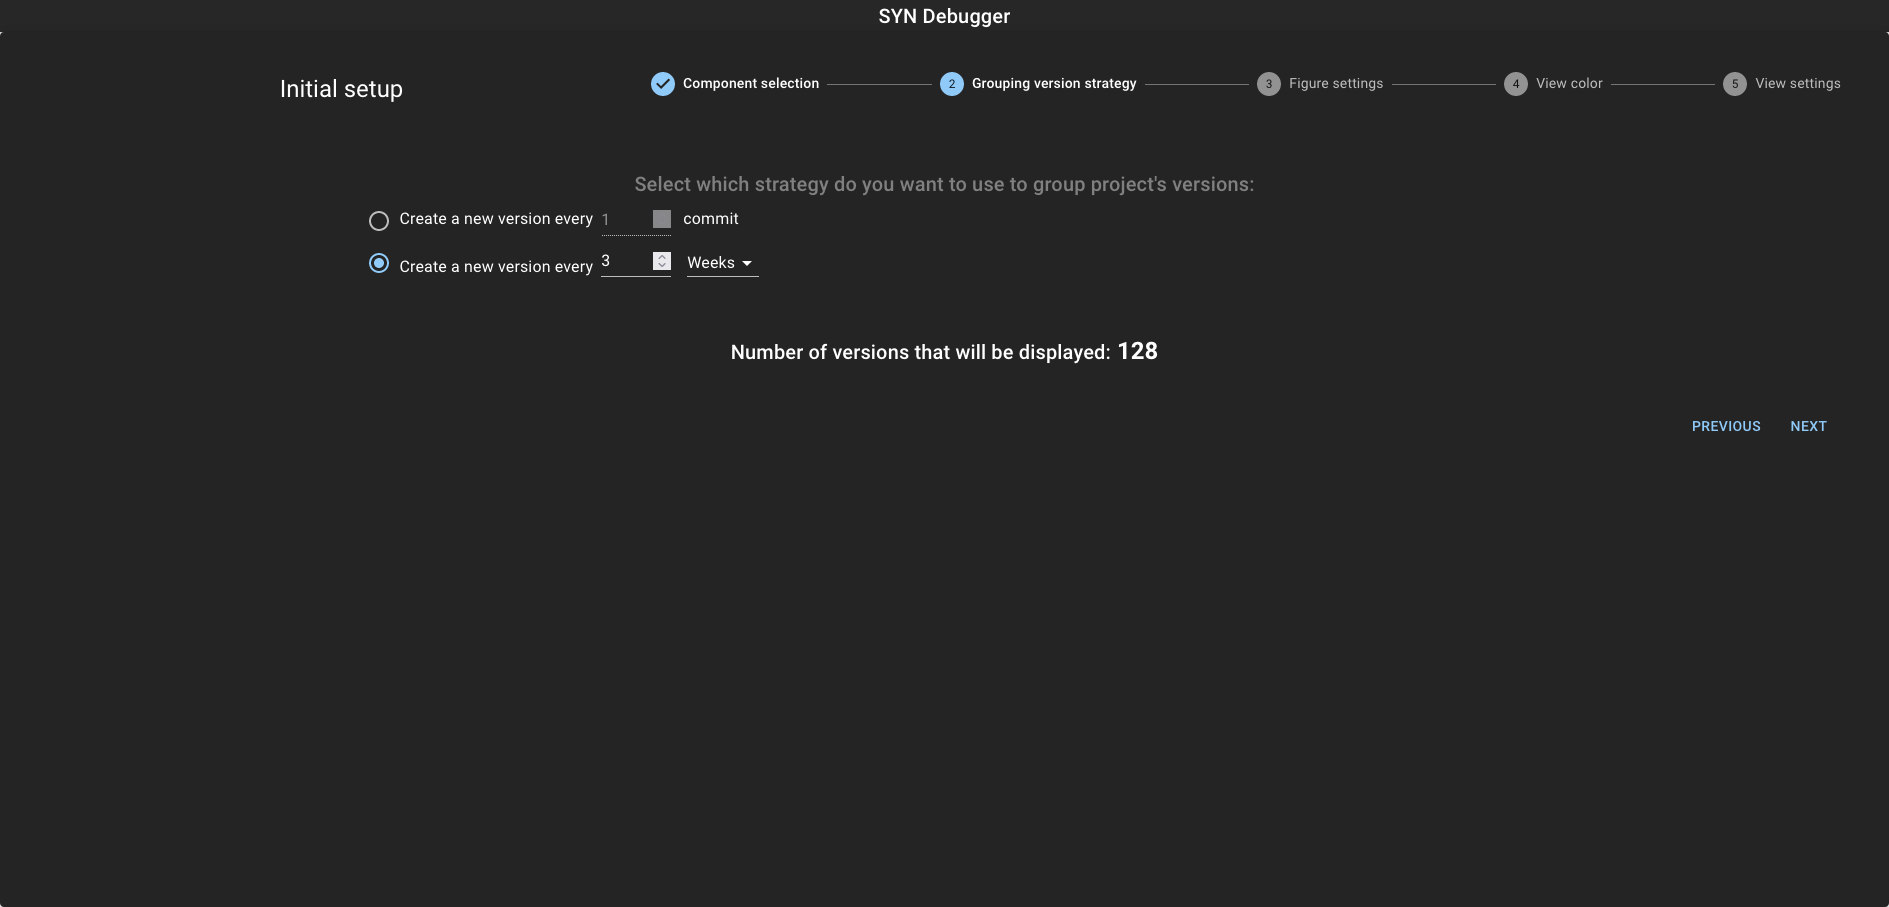
\includegraphics[width=\textwidth]{SYNUI-settings2.png}
    \caption{Project setup: grouping strategy}
    \label{fig:SYNUIsettings2}
\end{figure}

\subsubsection*{Figure settings}
The third step of the setup, shown in \autoref{fig:SYNUIsettings3}, allows the user to express graphical preferences. 
For each FileType selected in the step "Component selection", a card is created in this view. 
On each card user can customize:
\begin{itemize}
    \item which metrics should be considered by the visualization. These metrics are displayed when an entity is selected.
    \item the shape of the entity in the visualization. In our visualization, we implemented five shapes: BOX, TRIANGULAR, CONE, SPHERE, and CYLINDER. 
    \item the opacity of each FileType. 
\end{itemize}

Furthermore, the user can also express their preferences to choose which mapper strategies SYN must use to compute the height of entities, which metric must be used by the mapper, and the maximum height of the entities. 
The list of available metrics for the mapper comprises the metrics selected for each FileType.
Consequently, the UI has a checkbox to specify whether FileHistories that do not have the selected metric should be rendered or not. 
\bigbreak
With all the settings available on this page, the user has complete control over how FileHistories are rendered. 
There are a lot of possible combinations, each one with its purpose. For example, if we want a visualization that has a focus only on Java files, we can use the following settings:
\begin{itemize}
    \item BINARY metrics: none, shape: SPHERE, opacity: 0.3
    \item TEXT metrics: none, shape: SPHERE, opacity: 0.3
    \item JAVA metrics: SLOC, shape: BOX, opacity: 1
\end{itemize}
and for the mapper, use the LinearBucketValueStrategy, with the SLOC metric and a maximum height of 20. 

\begin{figure}
    \center
    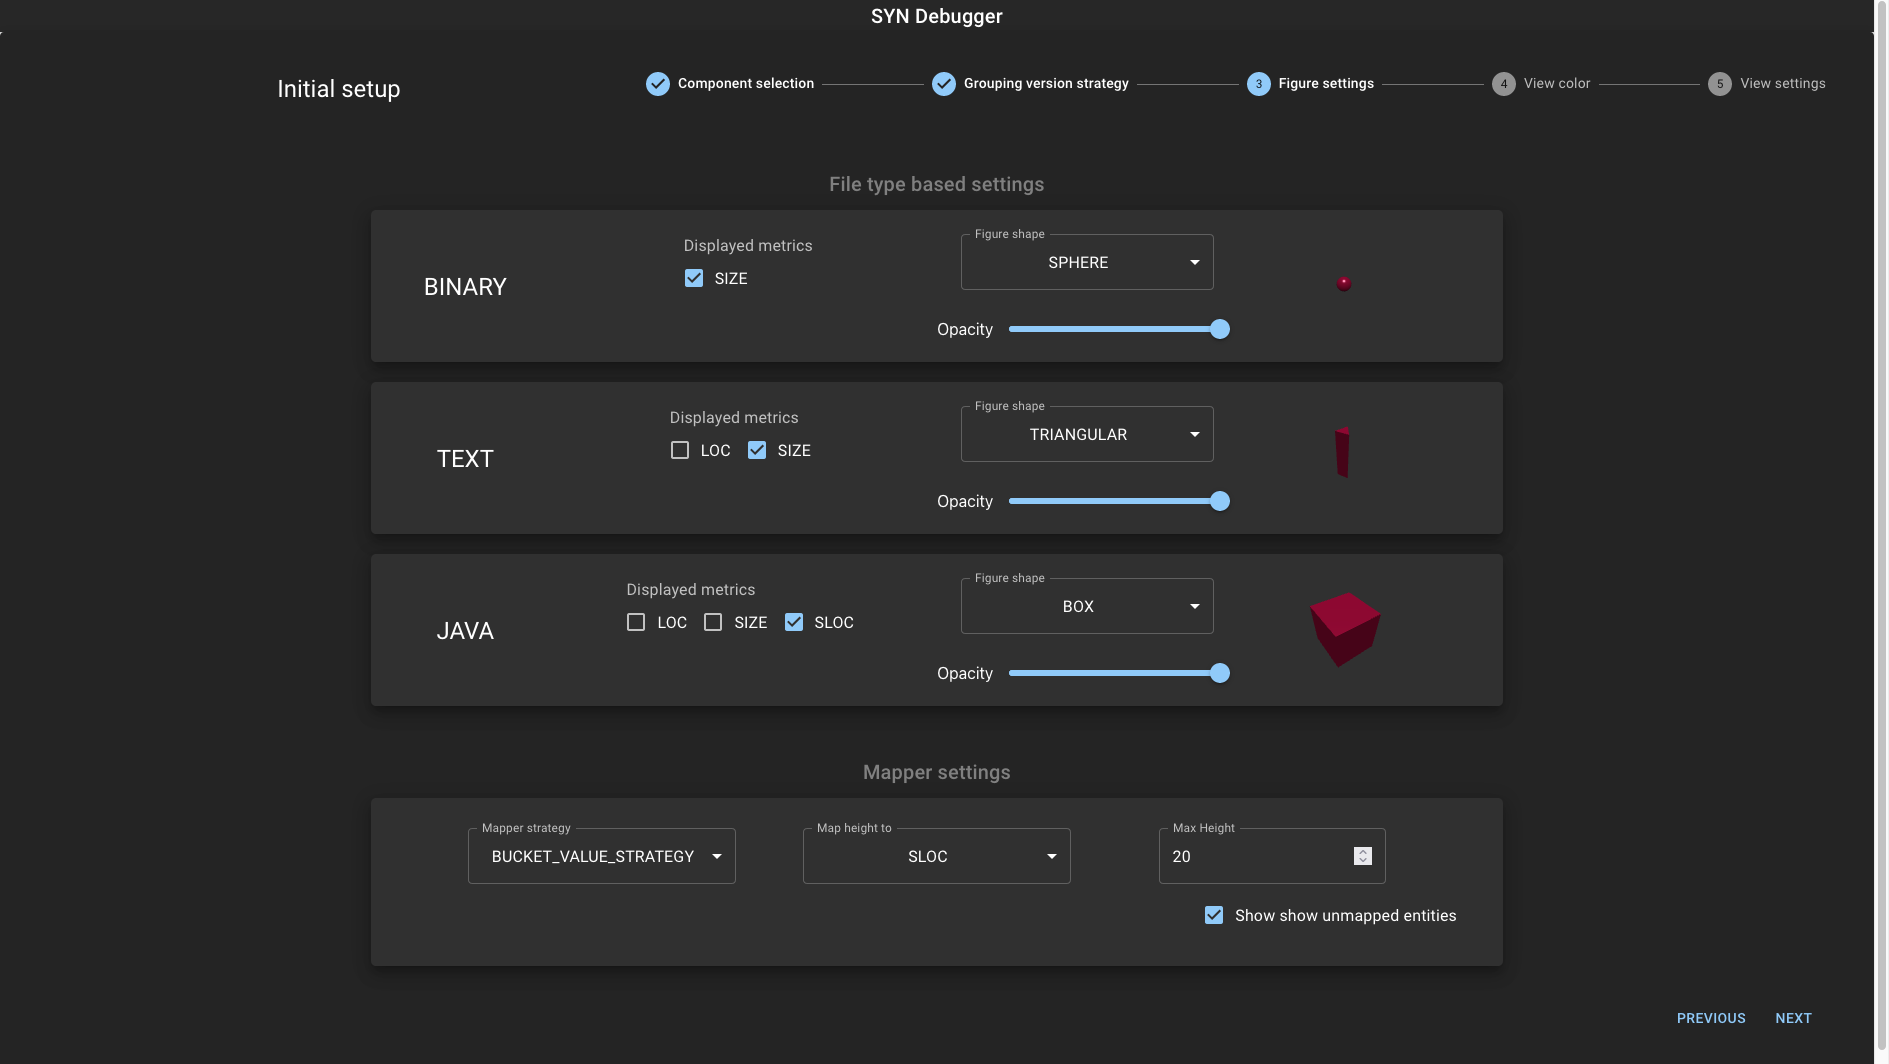
\includegraphics[width=\textwidth]{SYNUI-settings3.png}
    \caption{Project setup: figure settings}
    \label{fig:SYNUIsettings3}
\end{figure}

\subsubsection*{View color}
The fourth step of the setup, shown in \autoref{fig:SYNUIsettings4}, allows the user to express preferences about the color mapping of entities. 

The user has complete control over the way how aging is computed. 
As with grouping versions, aging can be done following two possible strategies: one by timestamp and one by commits. 
The color transition is linear. Therefore the user can choose the number of steps between the original color of the entity and the base color. 

Finally, each action has a distinct original color; the user can customize that. 

\begin{figure}
    \center
    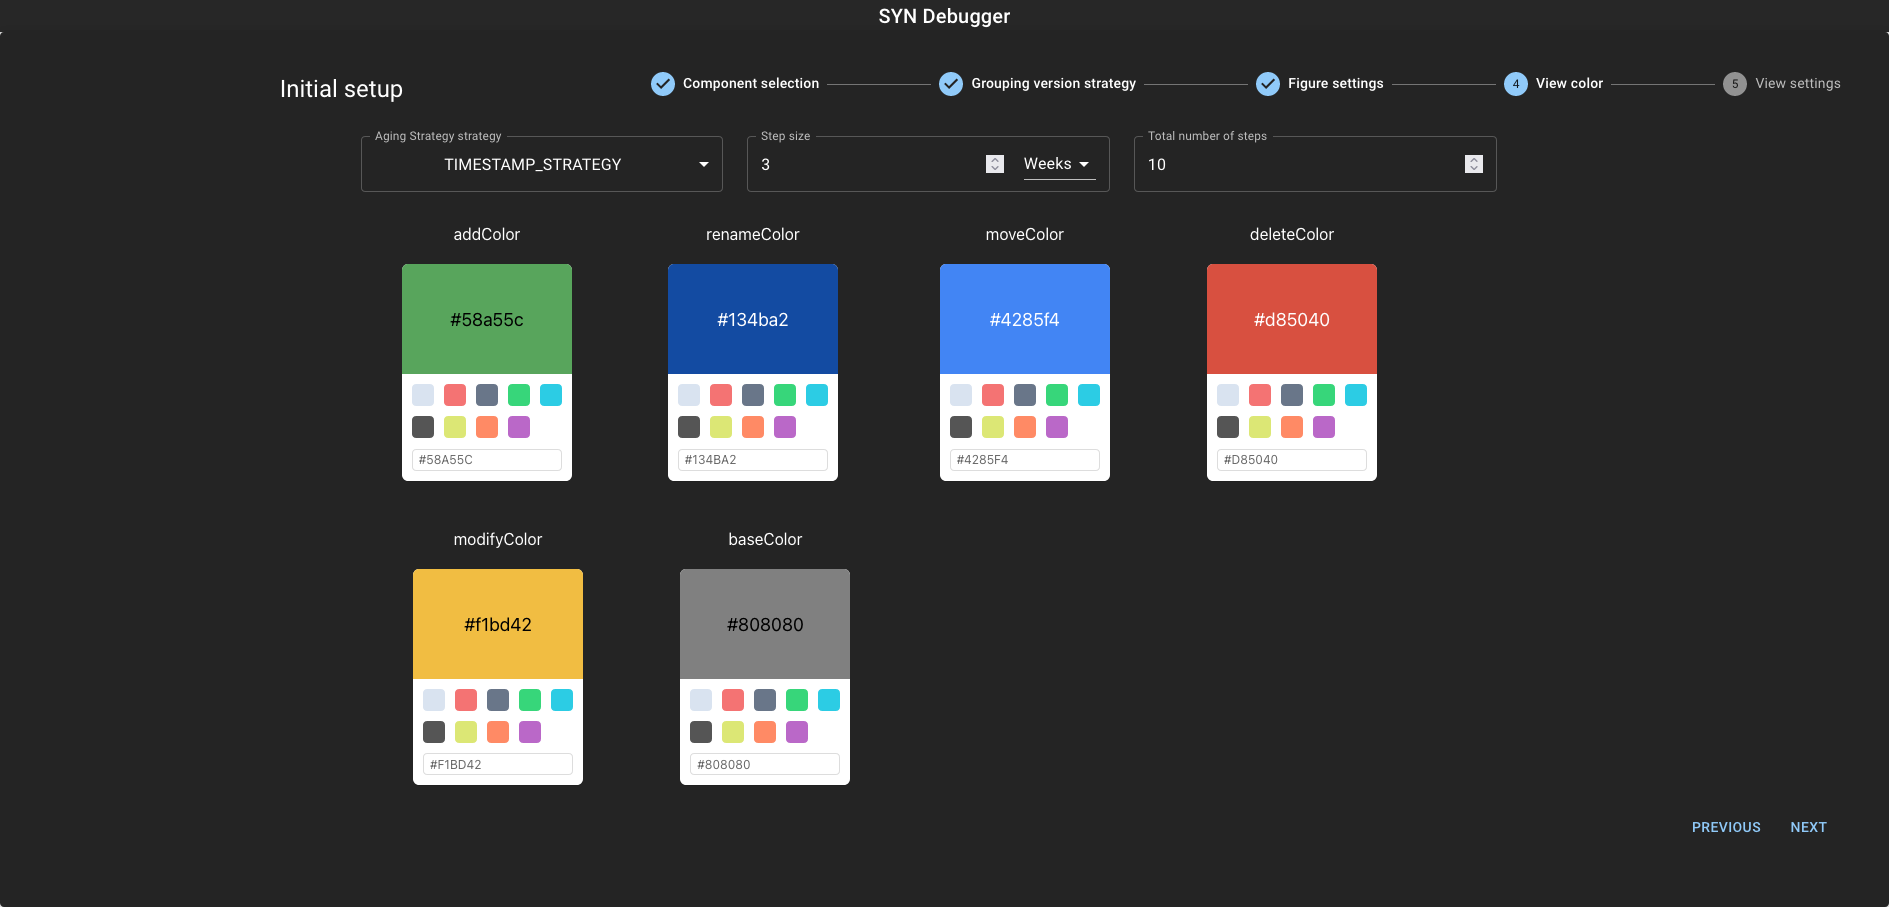
\includegraphics[width=\textwidth]{SYNUI-settings4.png}
    \caption{Project setup: view color}
    \label{fig:SYNUIsettings4}
\end{figure}

\subsubsection*{View settings}
The last step of the setup, shown in \autoref{fig:SYNUIsettings5}, allows the user to express general preferences about the behavior of the UI.

\begin{itemize}
    \item Show VR Button: if the UI should enable the full immersion experience that must be played with a VR headset. 
    \item Keep deleted entities: if the UI should keep deleted entities in the visualization. By default, these are not displayed. 
    \item Show debug layer: if the debugger of the 3D engine should be visible. 
    \item Auto screenshot: a screenshot should be automatically done once the UI is rendered.
    \item Shadows: if the UI should compute and render shadows. 
    \item Animation switching speed: the amount of time between the render of one animation and another if the autoplay button is pressed. 
\end{itemize}

\begin{figure}
    \center
    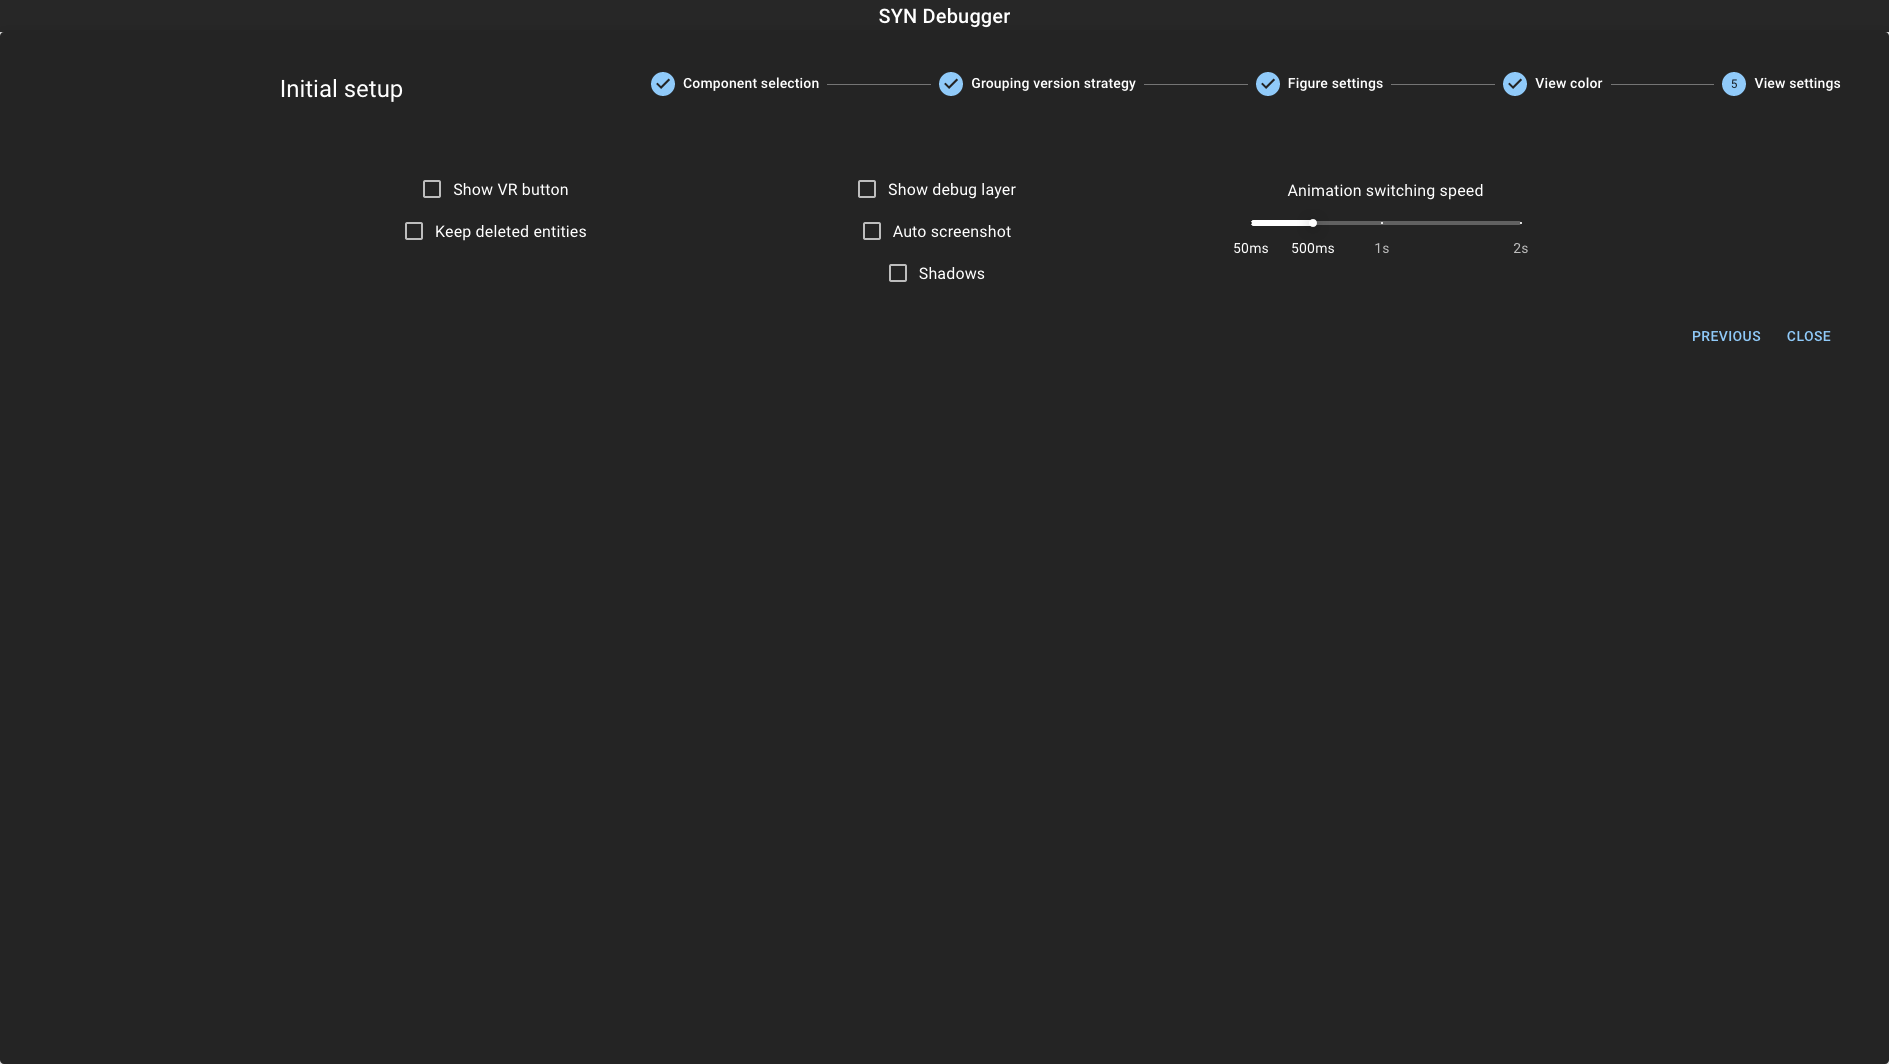
\includegraphics[width=\textwidth]{SYNUI-settings5.png}
    \caption{Project setup: view settings}
    \label{fig:SYNUIsettings5}
\end{figure}

\subsection*{Project visualization}
After having specified all the visualization preferences with the initial setup, they are stored in the web browser's local storage. 
Therefore, the UI can retrieve a view from the backend server, given the project id and the view specification. 

Initially, it calls the partialView query provided by the SYN-Server module. Once it gets the response, the visualization of the first AnimationFrame is automatically loaded. 
Since the partialView query returns only the first 100 AnimationFrames, to maximize the experience, a pre-fetcher mechanism was also implemented. 
One-half of the retrieved AnimationFrames have been displayed; it lazily requests a new partialView containing all the following AnimationFrames of the currently displayed view. 
In this way, the jump between a partialView and another is not subjected to network timing issues because the partial view was already prefetched. 
\bigbreak

The initial display of the view is represented in \autoref{fig:fileHistories}. The visualization settings of this view are:
\begin{itemize}
    \item Version grouping strategy: timestamp, three weeks
    \item Color palette: default
    \item Aging: timestamp, three weeks with ten steps
    \item Height mapper: BucketValueStrategy on SLOC
    \item Deleted entities are not shown
    \item All the entities have the same shape and opacity
    \item All the available metrics are selected for each FileType. 
\end{itemize}

The main visualization area can be broken down into four parts: 
In box A, a 3D environment displays FileHistories on a virtual plane. The camera is not fixed, and the view angle and the zoom level can be controlled with the mouse. 
In box B, we have a card that depicts the information about what the visualization shows to the user. 
This card includes the project's tile; the animation number displayed, the range of dates that this animationFrame has, and a list of commits included inside this AnimationFrame. This slider shows the overall progress of the display, and two buttons to jump to the next or the previous animation, and finally, one button to automatically jump to the following animation with the time interval previously set. 
Moreover, all the preferences specified during the project setup can be changed by clicking on the three dots in the top right corner.
In box C, we have a card to inform the user of the number of entities the UI renders. 
And finally, box D appears only when an entity is selected with the mouse. 
It has: 
\begin{itemize}
    \item the name and the current path of the entity. The current path is the entity's path on the last commit included in the displayed animation frame. 
    \item a table filled with all the metrics retrieved on the last commit of the displayed animation frame. The list of metrics is filtered with the one selected during the project setup. 
    \item a table filled with all the FileVersions associated with the selected FileHistory. For each FileVersion, the commit hash (clickable, automatically redirects to GitHub) and the action made on that commit are shown. Moreover, a tooltip with commit information appears if you hover on an action with the mouse.
    \item a contextual menu shown if you right-click on the card. With this contextual menu, you can jump on GitHub to see the raw file on the last commit of the currently displayed animation. 
\end{itemize}

\autoref{fig:deletedshadow} provides another visualization example where deleted entities are kept, and shadows are computed. 

\begin{figure}
    \center
    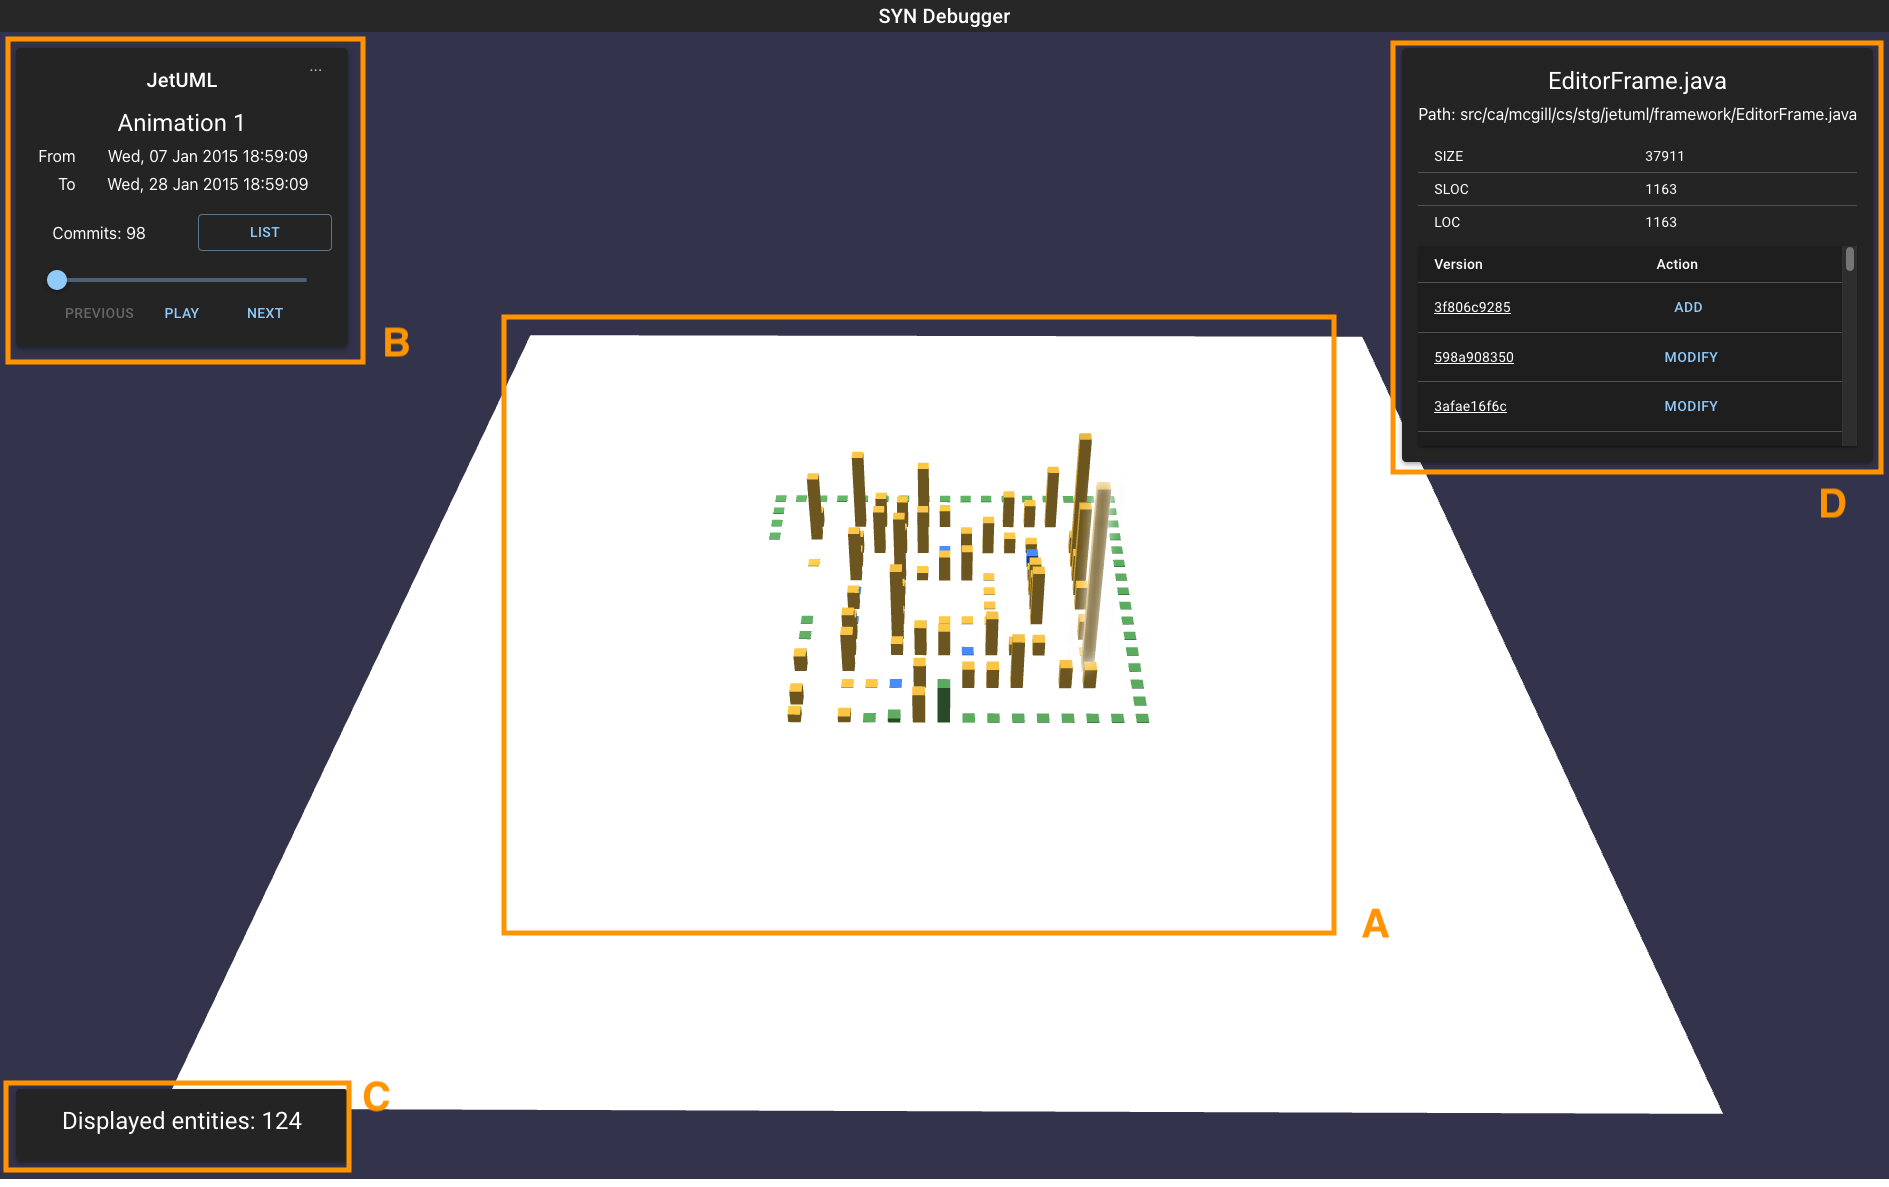
\includegraphics[width=\textwidth]{SYNUI-fileHistory.png}
    \caption{Visualization of JetUML with the default settings.}
    \label{fig:fileHistories}
\end{figure}

\begin{figure}
    \center
    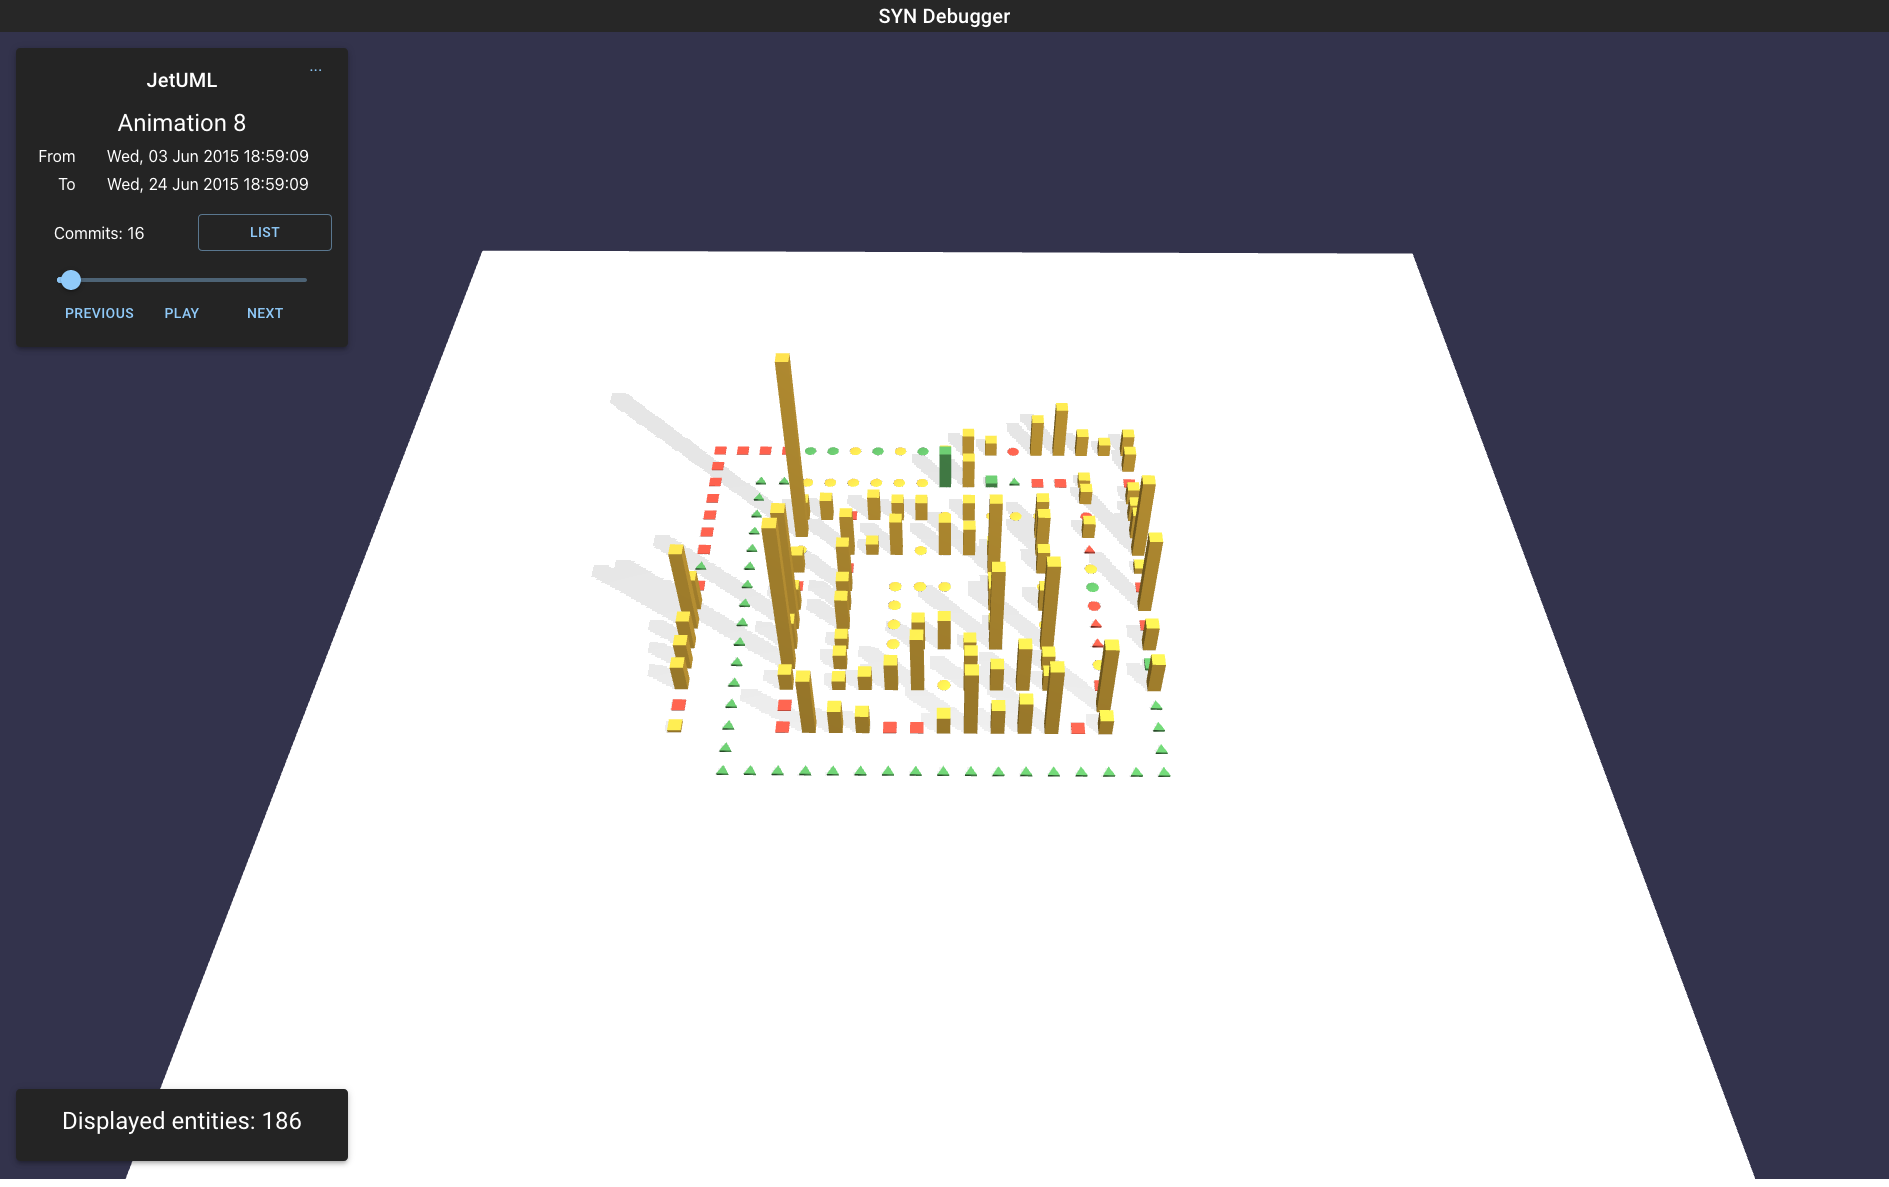
\includegraphics[width=\textwidth]{SYNUI-deletedshadow.png}
    \caption{Visualization of JetUML with shadows, deleted entities and custom shapes for non-java files.}
    \label{fig:deletedshadow}
\end{figure}

\bigbreak
SYN Debugger is a helpful tool to understand and debug the analysis process made with SYN. However, it has performance issues in rendering large systems. The main problem comes from the programming language chosen: Javascript. Since it runs on a web browser, it has limited resources available. Even though Javascript has APIs to support a high-performance rendering of 3D graphics \footnote{\url{https://developer.mozilla.org/en-US/docs/Web/API/WebGL_API}}, we experienced a significant FPS drop rendering large systems. To overcome this limitation and prove the versatility of our approach, we rendered large systems with POV-Ray \footnote{\url{http://www.povray.org}}. POV-Ray is an open-source tool for creating high-quality three-dimensional graphics. It works with \texttt{pov} files containing instructions to specify how the image should be rendered. We developed an extension of SYN that, given a View, produces a \texttt{pov} file for each AnimationFrame, following the same approach adopted in SYN Debugger.  